% !TeX spellcheck = en_US-architecture-part-1/
\chapter{Design and Architecture}

\section{Backend}

The backend needed to be able to handle multiple front-ends and a different data-storage option such as a database. There features needs to be available if for example User Story 8 was to be made, since it requires both a change in data-storage and user-interface.

An architecture matching these requirements are the Onion-Architecture. It was therefor used for overall architecture, this allows multiple front-ends while also abstacting away from the data, making it easy to switch to a database or other datasource.

The core namespaces can be seen in figure \vref{fig:Namespaces}, excluding testing and frontend namespaces.

\textbf{(Core) Domain Model}
 
The very center of the 'Onion', it should not reference anything other than itself. This is where all the models are defined, each model should also have an property called \textbf{Id} or ClassName\textbf{Id} so that the entity framework knows what to use as a key.

\textbf{(Core) Domain Services}

Is the 1st ring, it must only reference the Domain Model and nothing else. This is where all the interfaces to the Domain Model is, such as the Repository Interface.

\textbf{(Core) Application Services}

This is the outermost ring in the core, and is allowed to reference any core-libraries (Domain -Model and -Services).

\textbf{(Infrastructure) DataAccess}

Since it's outside the core, it's allowed to reference any libraries in the core. This is also where the ApplicationContext and Database Access can be defined. 

\textbf{Outer most ring}

This is where the frontends and testing frameworks will be, they can use any library.

\begin{figure}
	\centering
	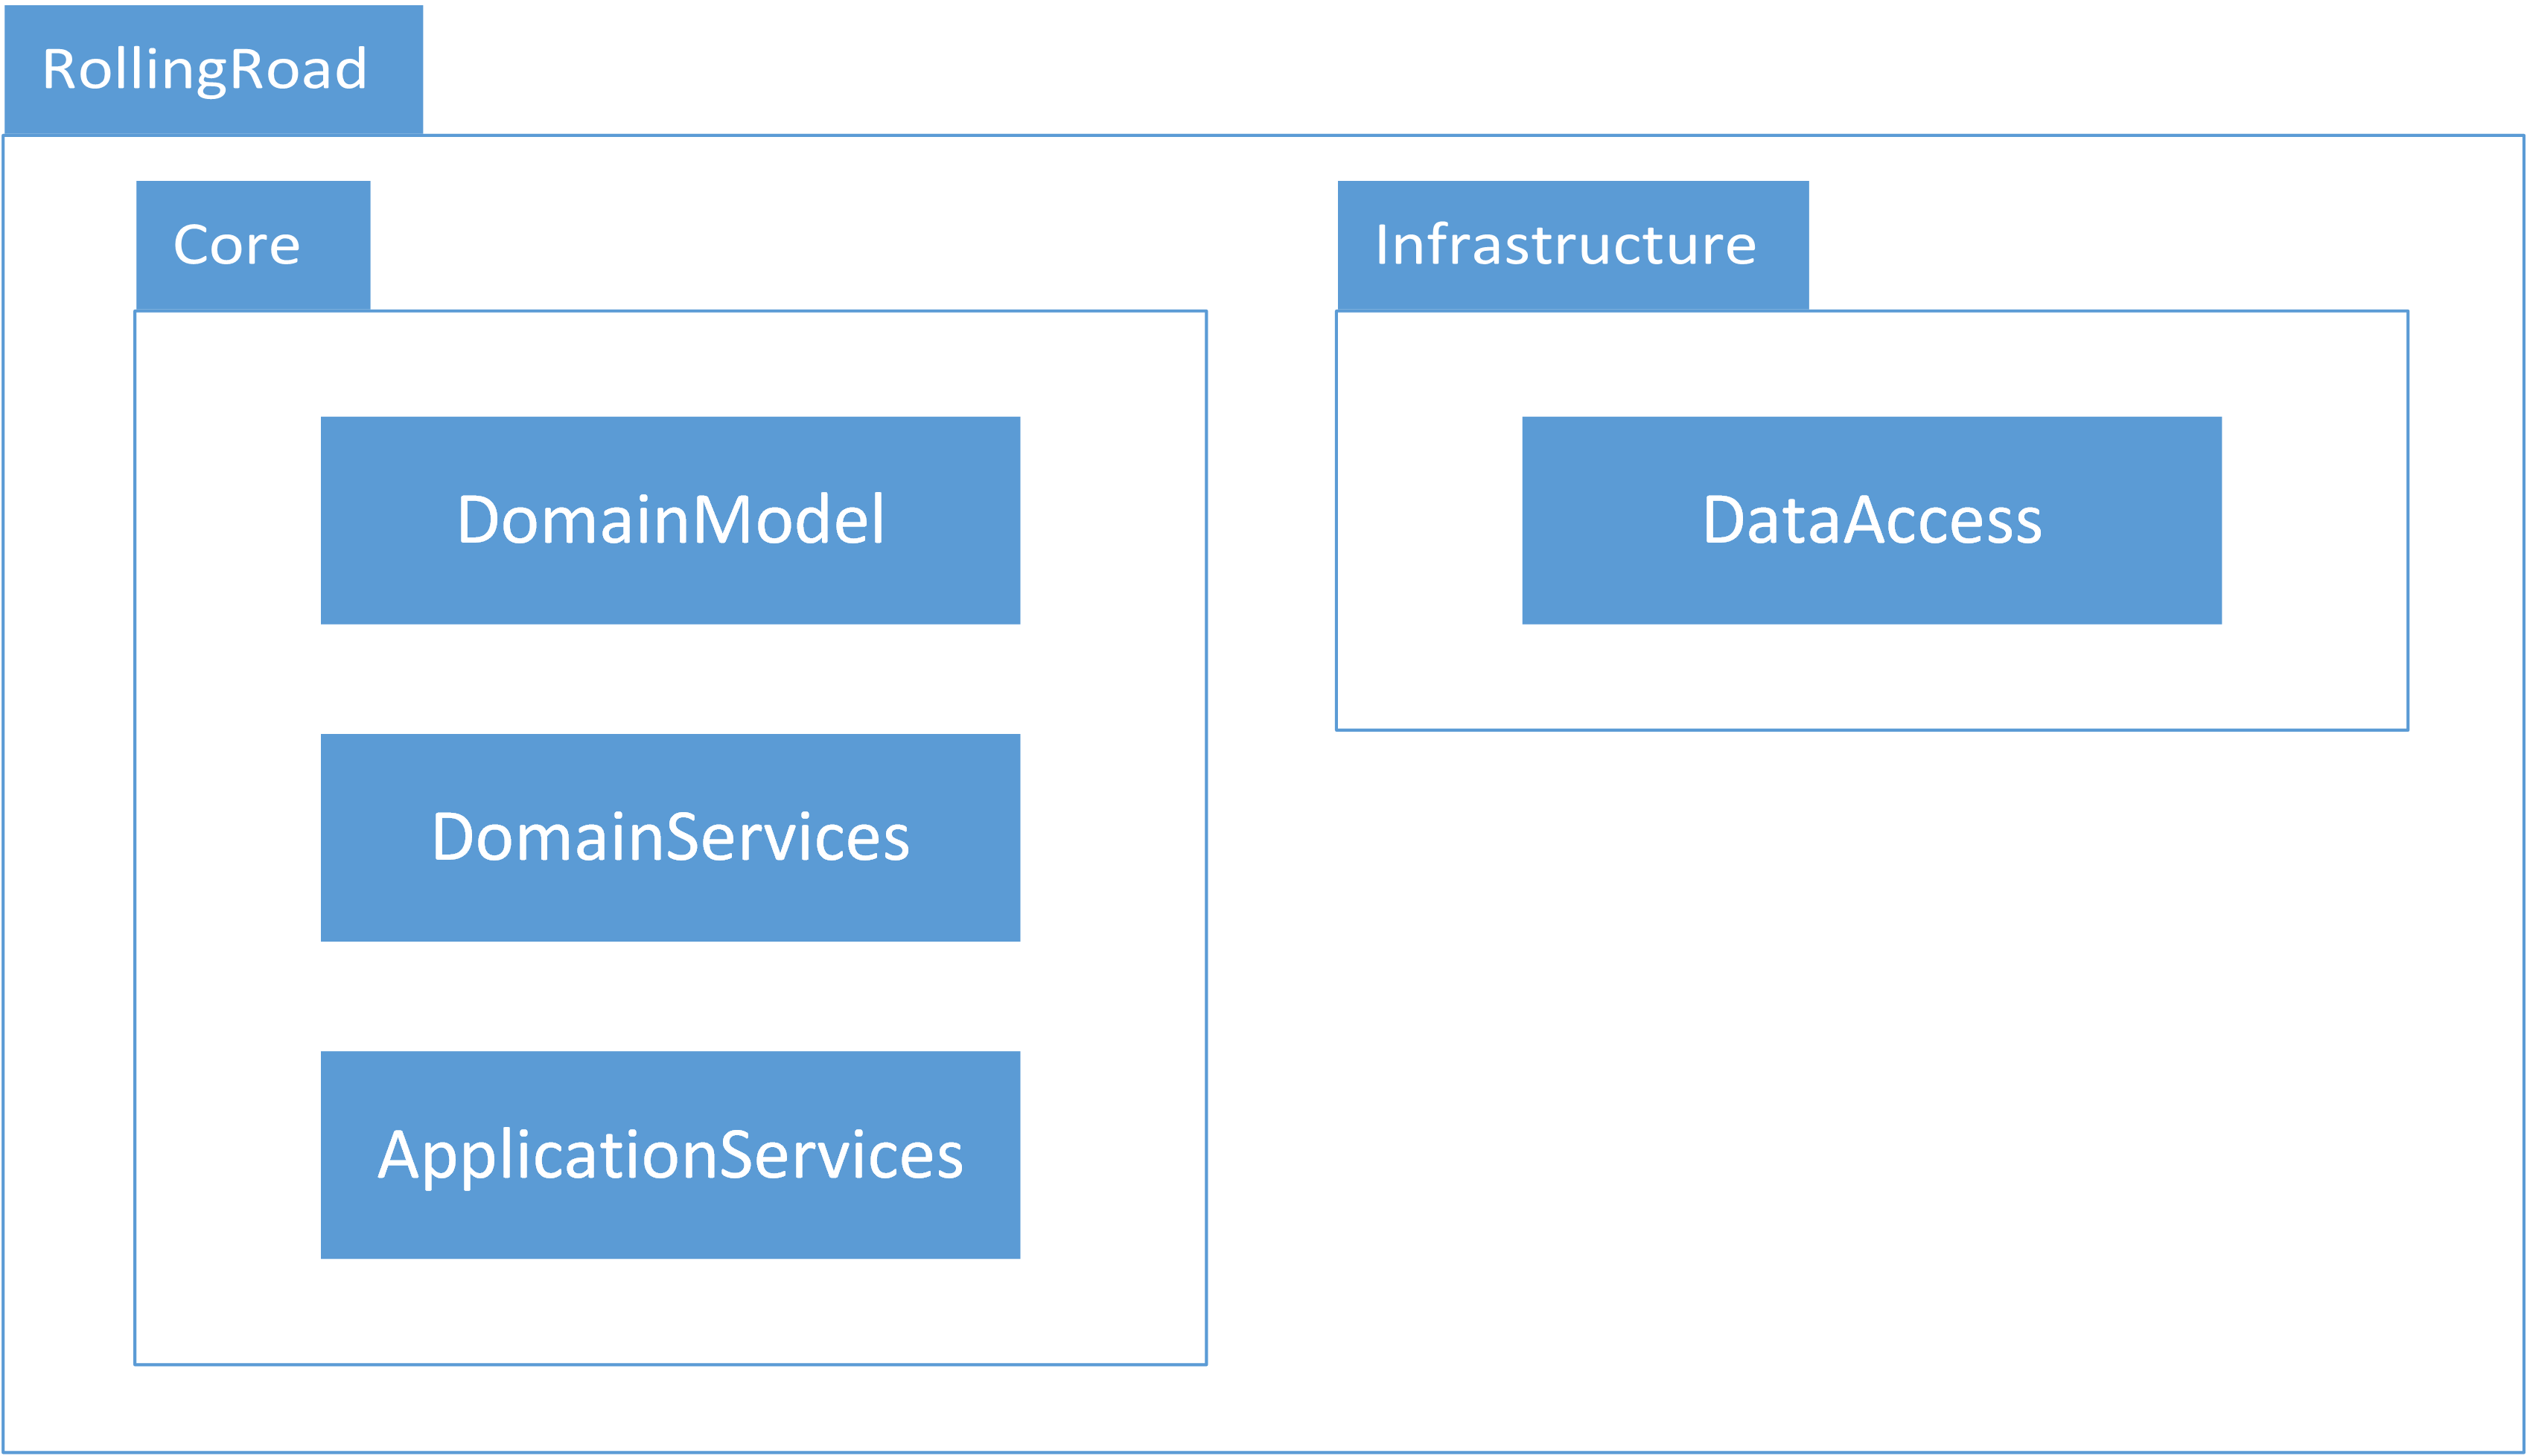
\includegraphics[width=0.7\linewidth]{Images/Namespaces}
	\caption{Main namespaces}
	\label{fig:Namespaces}
\end{figure}

\section{WPF-Application (Frontend)}

The frontend also has a ring in the Onion-Architecture called Presentation in this case, and in the RollingRoadGUI, is where the front-end WPF Windows application, on top of the onion architecture, MVVM(Model-View-ViewModel) was used to enabling unit testing.